\part{Subsistema de memoria}
\section{El sistema de memoria}
\subsection{Principio de vencidad o localidad}
\paragraph{Temporal Locality:} Una dirección de memoria que está siendo accedida actualmente tiene muy alta probabilidad de seguir siendo accedida en el futuro inmediato.

\paragraph{Spatial Locality:} Si actualmente se está accediendo a una dirección determinada de memoria, la probabilidad de que ésta y sus adyacentes sean accedidas en el futuro inmediato es muy alta.

La localidad de los programas surge naturalmente de su estructura. La mayoría contiene loops, osea que las instrucciones y los datos usados en ellos será accedido repetidamente lo que genera localidad temporal. Además, como son accedidas secuencialmente se tiene localidad espacial.

\subsection{Jerarquías de memoria}
Para aprovechar estos principios, se implementa la memoria de una computadora como una \textbf{jerarquía}. Ésta, consiste en múltiples niveles de memoria con diferentes tamaños y velocidades. Mientas más rápida sean, más caras por bit son. El objetivo es presentar al usuario con tanta memoria como sea posible con la tecnología más barata prooveyendo, al mismo tiempo, la velocidad de acceso provista por las memorias más rápidas.

En la actualidad, hay tres tipos de tecnologías usadas para construir las distintas jerarquías. La memoría principal es implementada con DRAM (Dynamic Random Acces Memory) mientras que los niveles más cercanos al procesador (caché) usan SRAM (Static Random Acces Memory)  [Ver sección \ref{sec::Memoria::Tipos}].

\begin{figure}[ht]
	\centering
	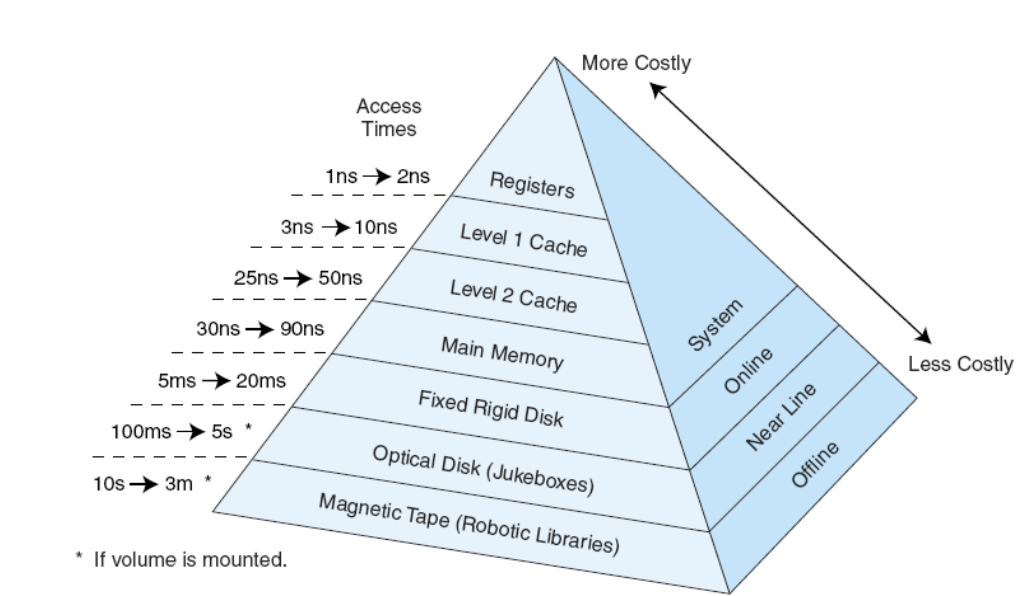
\includegraphics[width=1\textwidth]{imagenes/memory-heriarchy}
	\caption{Memory Hierarchy}
	\label{fig:memory-hierarchy}
\end{figure}

Sin importar el tamaño de la jerarquía, los datos son copiados solo entre dos niveles adyacentes. El nivel más alto - el más cercano al procesador - es más pequeño y rapido ya que usa tecnología más cara que el nivel más bajo.

\paragraph{Bloque:} La mínima unidad de información que puede estar presente en la jerarquía de dos niveles (la que está compuesta por las dos memorias que intercambian información).

\paragraph{Hit:} Se produce cuando la información pedida por el procesador se encuentra en algún bloque de la memoria que se está utilizando.

\paragraph{Miss:} Cuando la información debe ser buscada en el nivel inferior de la jerarquía.

\paragraph{Hit Rate:} La fracción de accesos a memoria encontrados en cada nivel1 de la jerarquía. A menudo es usado como medida de rendimiento de la misma.

\paragraph{Miss Rate: } 1 - hit rate (para cada nivel)

\paragraph{Hit time:} El tiempo que se tarda en acceder a un bloque en cada nivel de la jerarquía.

\paragraph{Miss penalty:} El tiempo requerido para fetchear un bloque desde el nivel inferior de la jerarquía (incluyendo tiempo de acceso, transmisión y copiado del bloque).

\newpage
\section{Tipos de memoria}\label{sec::Memoria::Tipos}
Hay dos tipos de memoria:


\begin{itemize}
	\item \textbf{No volátiles:} Son memorias capaces de retener la información almacenada cuando se les desconecta la alimentación. Son la tercera digievolución de las memorias \textbf{ROM} (Read Only Memory) que debían ser grabadas por el fabricante del chip y no eran modificables.
	
	De ROM pasaron a ser componentes programables que podían ser borrados con luz ultravioleta de una determinada longitud de onda. Y, luego, se convirtieron en las actuales memorias flash que pueden ser grabadas por algoritmos de escritura \textit{on the fly} por el usuario. El ejemplo más habitual son los discos de estado sólido de los equipos portátiles modernos.
	
	Se usan fundamentalmente para almacenar el programa de arranque de cualquier sistema.
	
	\item\textbf{Volatiles:} Conocidas como \textbf{RAM}, se caracterizan por que una vez interrumpida la alimentación eléctrica, la información que almacenaban se pierde.
	
	Estas memorias pueden almacenar mayores cantidades de información y modificarla en tiempo real a gran velocidad a comparación de las No Volátiles.
	
	Se clasifican de acuerdo con la tecnología y su diseño interno en:
	
	\begin{itemize}
		\item \textbf{Dinámicas (DRAM):} Almacenan la información en forma de una carga en un capacitor y la sostiene durante un breve lapso de tiempo con la ayuda de un transistor.
		
		Para guardar la información se activa el transistor que aplica el voltaje apropiado a la linea del bit. Una vez cargado el capacitor, se desactiva. 
		
		Después de un tiempo, la carga del capacitor (que se empieza a descargar) llega a un determinado threshold y en necesario volver a activar el transistor para cargar la información otra vez (si había un uno).
		
		Durante una operación de lectura, los capacitores de la celda seleccionada son activados y descargados completamente. En este caso, un amplificador detecta los valores leídos y aplica voltaje a las lineas de bits necesarias para volver a cargar
 		los capacitores necesarios. Esto aumenta el tiempo de acceso a la celda ya que no se puede liberar la operación hasta no haber repuesto el estado de carga de cada uno de ellos.
 		\item \textbf{Estáticas (SRAM):} Almacenan la información en un biestable. Una celda se compone de seis transitores (por lo que tienen menos capacidad por componente que las dinámicas).
 		
 		Tres de los seis transistores están saturados (conducen la máxima corriente posible de forma permanente) y los otros tres están al corte (conducen una corriente prácticamente insignificante pero no nula). Esto genera un mayor consumo de energía por celda.
 		
 		La lectura es directa y no destructiva lo que se traduce en un tiempo de acceso bajo en comparación con las memorias dinámicas.
	\end{itemize}

\end{itemize}

\newpage
\section{Memoria Caché}
Los niveles de caché son bancos de SRAM de muy alta velocidad que contienen una copia de los datos e instrucciones que están en memoria principal. Éstos, deben ser lo suficientemente grandes para que el procesador resuelva la mayor cantidad posible de búsquedas de código y datos en memoria asegurando una alta performance y lo suficientemente pequeñas para no afectar el consumo ni el costo del sistema.

Para implementar estas memorias se debe agregar un controlador que se encarga de mantener la caché actualizada y de indicarle que datos debe mandar al procesador.

\subsection{Operción de lectura}
\begin{itemize}
	\item El procesador inicia un ciclo de lectura de memoria, envía la dirección necesaria al controlador de caché.
	\item El controlador busca la dirección en el directorio de la caché.
	\begin{itemize}
		\item Si hay un \textbf{hit}, busca el ítem en la memoria caché y lo envía al procesador.
		\item Si hay un \textbf{miss},  busca el ítem en el sistema de memoria y lo copia en la caché. Actualiza el directorio de la misma y después manda la data al procesador.
	\end{itemize}
\end{itemize}

\begin{figure}[ht]
	\centering
	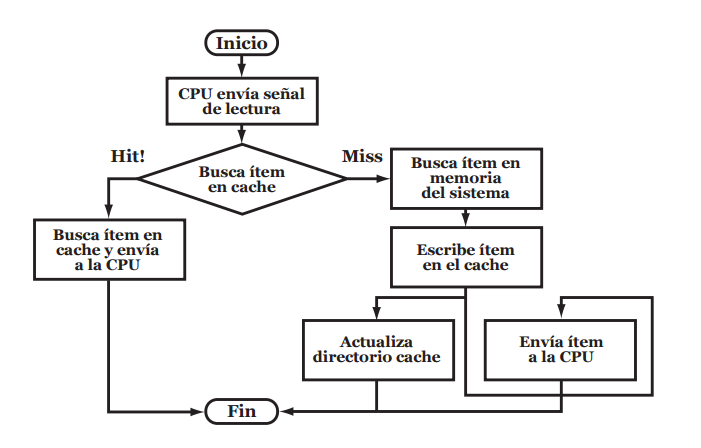
\includegraphics[width=1\textwidth]{imagenes/cache}
	\caption{Operación de lectura}
	\label{fig:reading-operation}
\end{figure}

\subsection{Organización de la caché}

\paragraph{Línea:} Elemento mínimo de palabra de datos dentro del caché. Corresponde a un múltiplo del tamaño de la palabra de datos de memoria. Esto nos permite copiar, en memoria, el ítem requerido y aquellos que lo rodean (principio de vecindad espacial).

\paragraph{Set:} Un conjunto que contiene $2^{ln}$ lineas de la caché.

\subsubsection{Mapeo directo}
Se divide, a la memoria en $2^j - 1$ paginas. Y cada página en $n$ bloques.

\begin{figure}[ht]
	\centering
	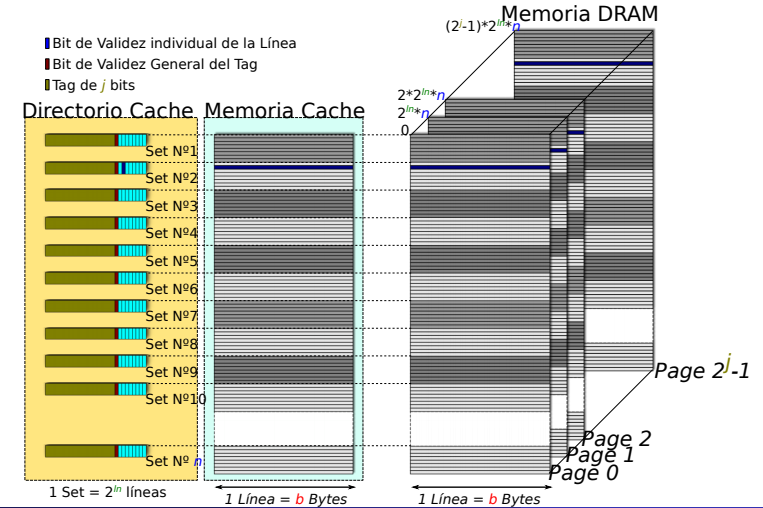
\includegraphics[width=0.75\textwidth]{imagenes/cache-mapeo-directo}
	\caption{Mapeo directo}
	\label{fig:direct-mapping}
\end{figure}
\begin{itemize}
	\item Los primeros $j$ bits de la dirección identifican la página a la que pertenece la línea.
	\item Los siguientes $n$, el set que les corresponde en la caché.
	\item Los $ln$ bits identifican la línea que le corresponde dentro del set
	\item y los últimos $b$ bits indican el índice de la palabra buscada dentro de la línea.
\end{itemize}

Para  buscar una dirección de memoria, en este tipo de caché:

\begin{itemize}
	\item Se busca el set en el que se encontraría esa dirección.
	\item Si el set tiene información válida, se corrobora que sea de la página de memoria a la que pertenece esa dirección.
	\begin{itemize}
		\item Si la página es correcta, entonces se accede al set en busca de la línea correspondiente y se vuelve el dato pédido.
		\item Sino, se trae de memoria un bloque de tamaño del set y remplaza el set actual por ese.
	\end{itemize}
\end{itemize}

\subsection{Asociativa de dos vías}

\begin{figure}[ht]
	\centering
	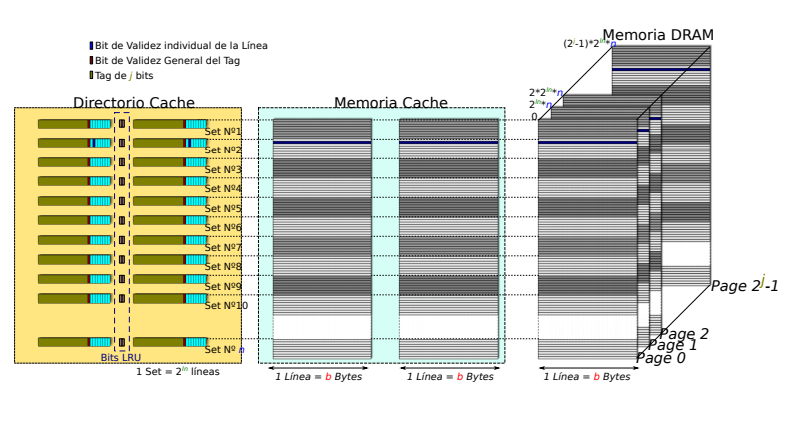
\includegraphics[width=0.75\textwidth]{imagenes/cache-asociativo-vias}
	\caption{Asociativo por 2 vías}
`	\label{fig:asociativo-mapping}
\end{figure}

Cuando se trae un bloque de memoria, éste puede ser copiado en cualquiera de las dos mitades mientras sea dentro del set correspondiente. Se utiliza un algoritmo (generalmente least recently used - LRU)) para decidir cual mitad remplazar con la nueva información.

\subsection{Operación de escritura (Coherencia de caché)}

Cuando modificamos un valor, sería ideal que el cambio se vea reflejado tanto en la caché como en memoria principal. Si esto no pasa, entonces diremos que las memorias son inconsistentes/incoherentes.

Dependiendo del sistema (si hay una sola CPU o más de una) se utilizan distintas \textbf{políticas de escritura}. Decidir cuál de ellas usar constituye una de las decisiones más importantes en el diseño del sistema de memoria:

\begin{itemize}
	\item \textbf{Write through:} Cada vez que hay que hay que modificar una dirección, el procesador manda el dato tanto a memoria príncipal como al controlador de la caché y se realiza la escritura en ambas memorias. 
	
	Esto garantiza coherencia entre ambos datos de manera absoluta pero penaliza cada escritura con el tiempo de acceso a DRAM. Osea que la performance se degrada durante estas operaciones.
	
	\item \textbf{Write through buffered:} El procesador manda la data al controlador de caché que la actualiza y sigue ejecutando instrucciones y usando datos de la misma.
	
	El controlador dispone de un buffer de escritura que va almacenando estas modificaciones mientras se espera a que sean escritas a memoria. Cuando la escritura finaliza, se desencola y sigue con la próxima modificación.
	
 	Si el buffer está lleno cuando el procesador pide una escritura, entonces se debe parar la ejecución y esperar a que tenga una entrada libre. Si bien la ocurrencia de los stalls es reducida, estos siguen pasando.
 	
 	\item \textbf{Copy back / Write back:} Se modifican solo las líneas de la caché y se marcan como \textbf{dirty} (modificadas). El controlador escribe el bloque en memoria cuando debe ser remplazada por otro. 
 	
 	Este método mejora el performance cuando el procesador puede generar escrituras tan o más rápido de lo que puede escribir en memoria. Sin embargo, es mucho más difícil de implementar.
\end{itemize}

Si el procesador realiza un miss mientras el controlador caché está accediendo a la DRAM, para actualizar el valor deberá esperar hasta que se termine la opreación para poder acceder a la misma.

\subsubsection{Coherencia en sistemas multi-procesador (Snoop Bus)}
El bus es un conjunto de cables que conecta varios dispositivos, cada uno de los cuales puede observar cada transacción del bus. Cuando un procesador emite un pedido a su caché, el controlador examina el estado de la misma y realiza las acciones adecuadas para completarlo. Esto puede generar transacciones para acceder a memoria.

En este caso, cada procesador posee una caché de primer nivel y todas ellas son conectadas al subsistema de memoria principal a través un único bus que es compartido. 

\begin{figure}[ht]
	\centering
	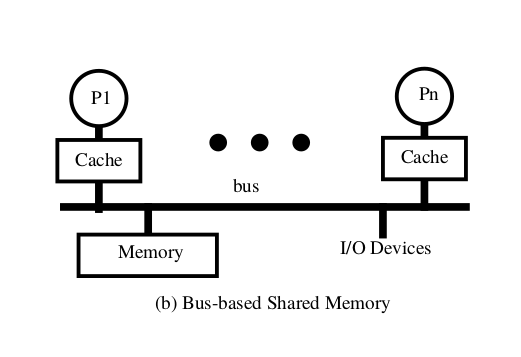
\includegraphics[width=0.5\textwidth]{imagenes/multiprocesor-caches}
	\caption{Bus de memoria compartido}
	\label{fig:busCompartido}
\end{figure}

Cuando un procesador modifica un bloque de memoria presente en su caché, se produce una incoherencia en las caches de los otros procesadores que tenían su propia copia del bloque. Esto sucede porque la misma contiene un valor obsoleto en la dirección de memoria modificada por el primer procesador.

%\paragraph{Coherencia (en multiprocesadores):} Un sistema de memoria es coherente si es posible, para toda dirección, construir un orden serial de todas las operaciones que acceden a ella tal que:
%\begin{itemize}
%	\item Es consistente con los resultados de le ejecución.
%	\item Las operaciones emitidas por un procesador ocurren en el orden que fueron producidas por el mismo.
%	\item El valor devuelto por cada lectura es el valor escrito por la última operación de escritura en ese orden.
%\end{itemize}
%
%Está implícita, en esta definición, la propiedad de \textbf{serialización de escritura}. Ésta nos asegura que todos los procesadores ven todas las escrituras a una dirección en el mismo orden.

%\paragraph{Snooping bus:}
La coherencia se mantiene haciendo que cada controlador de caché espíe el bus y monitoreé las transacciones. El controlador del bus funciona como arbitro para  decidir el orden en el que estas son ejecutadas. Cuando una transacción es enviada por el bus, se envia la dirección a la que se está accediendo y el tipo de operación que se está realizando sobre ella.

Cada controlador de cache, toma la dirección enviada por el bus y chequea si tiene una copia del bloque referenciado por la misma.

\begin{itemize}
	\item \textbf{con write-through:} Todas las escrituras se realizan directamente en la memoria principal. Todas las caches que tengan una copia del bloque modificado invalidan esa entrada. De esta forma, cuando el procesador necesite leer esa dirección, se tendrá que volver a cargar el bloque desde la memoria principal.
	
	El problema con este método es que se accede a memoria por cada operación de almacenamiento.
	
	\item  \textbf{write-back:} Al momento, es el método más utilizado ya que reduce drásticamente estos accesos. Sin embargo, no puede ser usado directamente en estos sistemas ya que no sería posible identificar donde está el último valor válido de una dirección. Por esta razón, se desarrollaron protocolos de coherencias (el más popular de ellos M.E.S.I) que nos permiten identificar la validez de nuestros datos.
\end{itemize}

\subsubsection{Protocolo MESI}
En este protocolo, un bloque de memoria en la caché puede estar en cuatro estados:

\begin{figure}[ht]
	\centering
	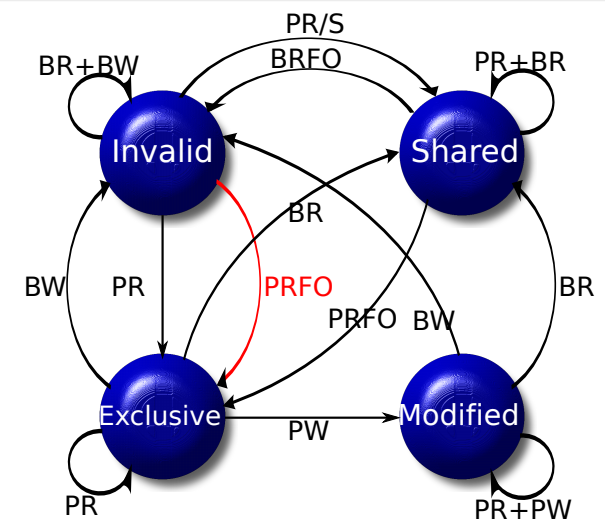
\includegraphics[width=0.5\textwidth]{imagenes/mesi-state-graph}
	\caption{Diagrama de estados de MESI}
	\label{fig:mesiDiagram}
\end{figure}

\begin{itemize}
	\item \textbf{Modified (M):} Es la única copia valida. La memoria principal está desactualizada y ninguna otra caché tiene una copia valida del mismo bloque.
	\item \textbf{Exclusive (E):} Esa caché es la única que contiene una copia de ese bloque. Además, esa copia no está modificada.
	\item \textbf{Shared (S):} Está presente en esa caché sin ninguna modificación, la memoria principal está actualizada y puede haber otra caché que también lo tenga.
	\item \textbf{Invalid (I):} No está presente en la caché o contiene información desactualizada.
\end{itemize}

\paragraph{Lectura de un bloque:}
Supongamos que el procesador necesita leer un bloque de memoria, entonces produce un processor read (\textbf{PR}):
\begin{itemize}
	\item Si el bloque esta en caché (\textbf{Modified}, \textbf{Exclusive} o \textbf{Shared}), se resuelve el pedido.
	\item Si el bloque es \textbf{Invalid} entonces se genera un busRead (\textbf{BR}) y todas las cachés responden con una señal indicando si tienen o no una copia del valor pedido:
	\begin{itemize}
		\item Si no está en ninguna otra caché, se lo carga en modo \textbf{Exclusive} desde memoria principal.
		\item Si lo tiene alguna otra, se copia el bloque en modo \textbf{shared} después de haber tomado las medidas necesarias para mantener la consistencia. Si la otra caché lo tiene:
		\begin{itemize}
			\item En modo \textbf{Exclusive}, se lo pasa a estado \textbf{Shared}.
			\item En modo \textbf{Modified}, se copian a memoria principal los cambios realizados y se lo pasa a \textbf{Shared}
			\item En modo \textbf{Shared}, no se hace nada.
		\end{itemize}
	\end{itemize}
\end{itemize}

\paragraph{Escritura de un bloque:} Para escribir en un bloque, el procesador primero debe asegurarse que es el único con permisos de escritura, entonces:

\begin{itemize}
	\item Si el dato está en caché en modo \textbf{Modified} o \textbf{Exclusive}, genera un processor write (\textbf{PW}) y se modifica la caché. En el segundo caso, se pasa al estado \textbf{Modified}.
	\item Si está en \textbf{Invalid} ó \textbf{Shared}:
	\begin{itemize}
		\item Genera un Processor Request For Ownership (\textbf{PRFO}), pasa el bloque a estado \textbf{Exlusive} y todas las otras cachés invaliden sus copias.
		\item Luego, genera el proccesor write (\textbf{PW}), realiza las modificaciones y pasa el bloque a \textbf{Modified}
	\end{itemize}
\end{itemize}